\chapter{Study}

\section{Motivations}

%From our exploratory study, we were able to obtain a significant but weak effect between disclosing the source and the levels of trust marked by readers towards an article.

% We also observed trends that suggested an interaction between disclosing the source and the reading level of a story.

% However, the study faced several limitations: first, we did not obtain enough samples to show a statistically significant result for interactions between source and reading level.

% Furthermore, multiple levels of independent variables (ie: 5 levels for input source) made modeling complex and the results less clear.

% The dataset was also unbalanced and sparse (ie, because of large numbers of input variables we did not have complete representation for each category, such as high, low, and mid-reading level stories for every outlet and topic). We tried to control for those factors by randomization, however it made more difficult to analyze specific correlations between source and trust.

% To further explore the interaction between disclosing the source and the reading level of the story, we set up another crowdsourcing experiment on CrowdFlower, this time targeting this specific interaction, to see if there is a significant effect between the two, detailed in the following chapter.
 
This study sets out to tackle the question of reading level's effect in perceptions of news bias. In particular, how does it compare to factors associated with latent biases of the reader, such as media brand?

Although the body of literature in Chapter 2 examines the theories behind partisanship and media branding, little work has been done to compare those contextual effects with the effects of \emph{content} within a story, such as language use.

This thesis tests six hypothesis.

We explore two novel hypotheses testing reading level effects:

\begin{itemize}
\item \textbf{H1}: High reading level stories increase trust in the story.
\item \textbf{H2}: However, they decrease perceptions of fairness. 
\end{itemize}

As well as two comparing the role of \emph{content} versus \emph{context}:

\begin{itemize}
\item \textbf{H3}: Media brand has a stronger role in determining story trust than the content. 
\item \textbf{H4}: Media brand has a stronger role in determining story fairness than the content.
\end{itemize}

And two verifying former theories:
\begin{itemize}
\item \textbf{H5}: Stories shown to be from outlets of aligned political party score significantly higher on both trust and fairness than those of the opposite.
\item \textbf{H6}: Stories about candidates opposite to the readers preferred candidate score significantly lower in fairness, regardless of outlet.
\end{itemize}

We hypothesis \textbf{H1}: that high reading level of stories increase trust based off the work from Weisberg et. al showing that neuroscience explanations sway believability of scientific explanations, due to the field-specific nature of political reporting \cite{weisberg2008seductive}.

Conversely, we predict \textbf{H2} that it creates a decrease in the perception of fairness in the story, due to the polarizing nature of political news and the fact that more complex stories could cause a partisan individual to more quickly reject what appears as an onslaught of conflicting information \cite{cacioppo1979effects}.
 
 We hypothesize \textbf{H3} and \textbf{H4} that media brand effects outweigh content in determining both trust and fairness.

 Finally, we expect to see hostile media effects (\textbf{H5} and \textbf{H6}) to emerge.

\section{Experimental Design}
%For the second study, our experiment was revised to have a 4 x 2 mixed-factorial design.
Our experiment has a 4 x 2 mixed-factorial design.

In this study, reading level of articles and candidates featured in the articles were treated as within-subject variables, and the source of the story between-subjects.
\newpage
\begin{center}
\begin{table}
\begin{tabular}{ | m{10em} | m{7em}| m{7em} | m{7em} | m{7em} | } 
 \hline
  & \textbf{Source: None} & \textbf{Source: AP} & \textbf{Source: Fox} & \textbf{Source: CNN} \\
 \hline
 \textbf{High Reading Level} & Clinton, Cruz, Sanders, Trump & Clinton, Cruz, Sanders, Trump & Clinton, Cruz, Sanders, Trump & Clinton, Cruz, Sanders, Trump  \\ 
 \textbf{Low Reading Level} & Clinton, Cruz, Sanders, Trump & Clinton, Cruz, Sanders, Trump & Clinton, Cruz, Sanders, Trump & Clinton, Cruz, Sanders, Trump \\ 
 \hline
\end{tabular}
\caption{Main Study Design}
\label{study2}
\end{table}
\end{center}
%\newpage

% \begin{itemize}
%   \item Source (4 levels: None, AP, CNN, Fox)
%   \item Candidate (4 levels: Clinton, Cruz, Sanders, Trump)
%   \item Reading Level (2 levels: High, Low)
% \end{itemize}

This time, we reduced the number of stories to N=8, and also changed reading level from a 3-level to 2-level variable (low, high) for clarity.

Most significantly, since we observed some significant effect from disclosing source to the reader in Study 1, we added a manipulation in this experiment to further study the effect of revealing the source:

Following Baum's research in showing the effects of media brands and reader bias by manipulating reported brands, all eight stories in Study 2 were in fact written by the Associated Press, however, we manipulated the source shown to the reader \cite{baum2008eye}. In group A, readers were shown the headline and text of the story with no other context. In group B, readers were additionally shown that the story was from the Associated Press (true label). In groups C and D, readers were shown that the story was from CNN and Fox News, respectively.

This setup was created to eliminate some of the confounding effects from using stories from different sources (writing style, focus of content, slant, etc.), while directly observing the effect of revealing a specific source to the reader. The Associated Press was chosen as the source of the stories as it is the highest circulation newswire service in the United States, and has 14,000 members that use its content \cite{apFAQ}. Notably, both CNN and Fox News publish content in full or part from the Associated Press, although the specific stories chosen had not been published in full by either to avoid bias.

We removed the favorability question from Study 1 (as the 3-point scale did not yield significant results), instead asking the reader more directly about media bias by ranking the fairness of the story on a 5-point Likert scale. The trustworthiness question from Study 1 was kept, also on the same 5-point Likert scale.


\subsection{Dataset} 
Eight stories were chosen for this study: two (high and low reading level) per candidate. All eight stories were written by reporters from the Associated Press (although they may have been republished elsewhere).

Reading level cutoffs were made by taking the bottom and top 25\% percentile of Flesch-Kincaid scores for each candidate. From stories written by the Associated Press that made the cutoff, we formed pairs of high and low reading level stories from each topic. The topic with the highest distance between reading level in the pair was chosen for each candidate.

% put histograms of reading level with cutoff lines

 
 
 
\subsection{Survey}


\begin{figure}[h!] 
\centering
  \frame{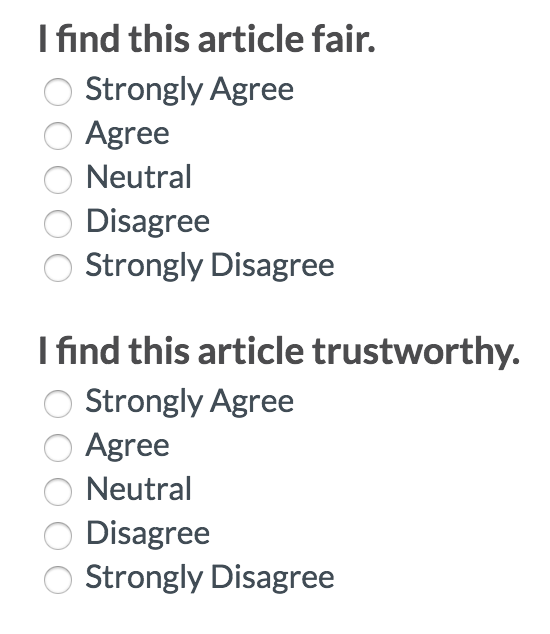
\includegraphics[width=0.45\textwidth]{study2_qs}}
  \caption{Survey Questions for Study 2}
\end{figure}



% Demographics
% What is your gender?
%  Male
%  Female
%  Other
% What is your age?
%  18-29
%  30-49
%  50-64
%  64+
% What is your political party affiliation?
%  Democrat
%  Republican
%  Independent/Other
%  No Affiliation
% If the election were tomorrow, I would vote for…
%  Hillary Clinton
%  Bernie Sanders
%  Donald Trump
%  Ted Cruz
%  John Kasich
%  Other
%  Might not vote
% Have you read any of the stories above before this study?
%  Yes
%  No
%  Might have, but I am not sure


 % when we removed people who might have already read stories, no sig diff results in analysis.



% just pics etc. 

\subsection{Quality Control}

CrowdFlower has a built-in ``Test Question'' feature that allows for the rejection of a annotator whose answers to specific questions do not lie within a threshold (default 70\%) of the ``correct'' answer or whose answers lay outside the standard variation compared to others.

However, since the questions we asked were by nature subjective and therefore outliers and disagreements in answers could imply signal rather than noise, we chose to monitor for quality using other metrics instead. CrowdFlower was not designed explicitly for survey-like tasks, and therefore there were no options for different screening methods or questions. Gold Questions on the platform are selected by the creator within the set of all questions being recorded.

Because of this, we monitored quality of results in two ways:

First, by setting a minimum of time of 360 seconds to complete the task of reading 5 stories for a task to be accepted.

Second, by selecting only Level 3 contributors on CrowdFlower as suggested on their website for handling survey-like tasks \cite{CrowdFlower-guide}.

Level 3 contributors are described as those who ``have completed over a hundred Test Questions across hundreds of different Job types, and have a near perfect overall Accuracy'' \cite{CrowdFlower-levels}. This is the highest category of contributor.
 
Users were also only allowed to answer the set of questions once. 

\$0.80 was given per survey, as suggested by MIT Committee on the Use of Humans as Experimental Subjects. The average response time per survey was 09:20 min.


\section{Basic Analysis}


\subsection{Demographics}


% \begin{figure}[h!] 
% \centering
%   \frame{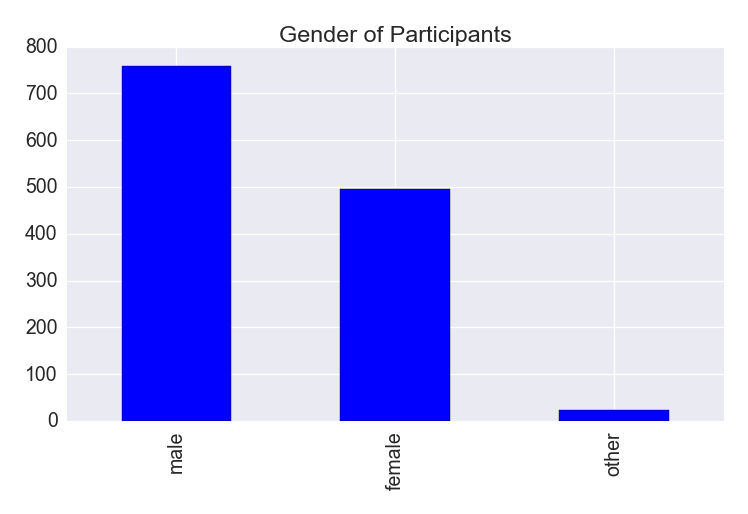
\includegraphics[width=0.45\textwidth]{gender_study2}}
%   \caption{Survey Questions for Study 2}
% \end{figure} 

See figure~\ref{fig:demographics2} on page \pageref{fig:demographics2}

See figure~\ref{fig:locations2}
See figure~\ref{fig:party2}

% \begin{figure}[h!] 
% \label{fig:demographics2}
% \centering 
%   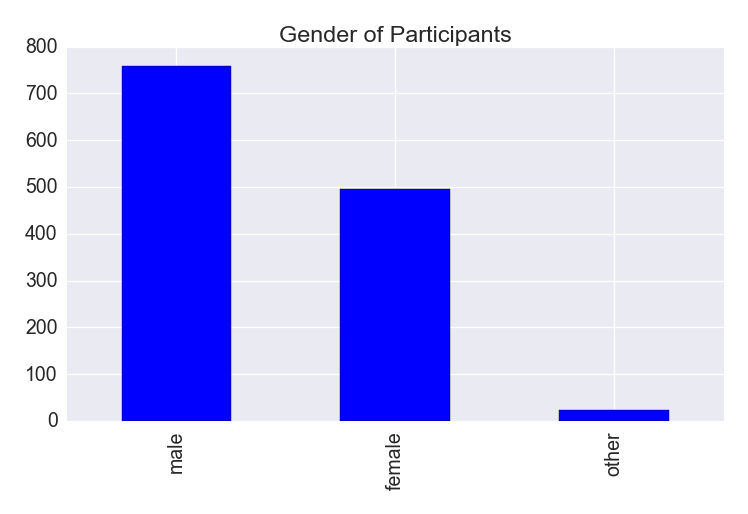
\includegraphics[width=0.8\textwidth]{gender_study2} 
%   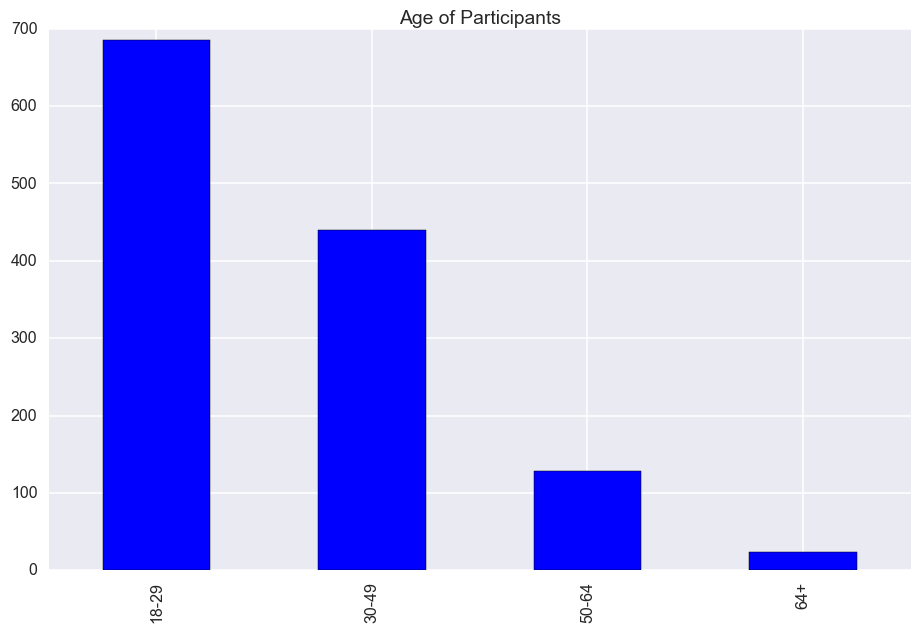
\includegraphics[width=0.8\textwidth]{age_study2} 
%   %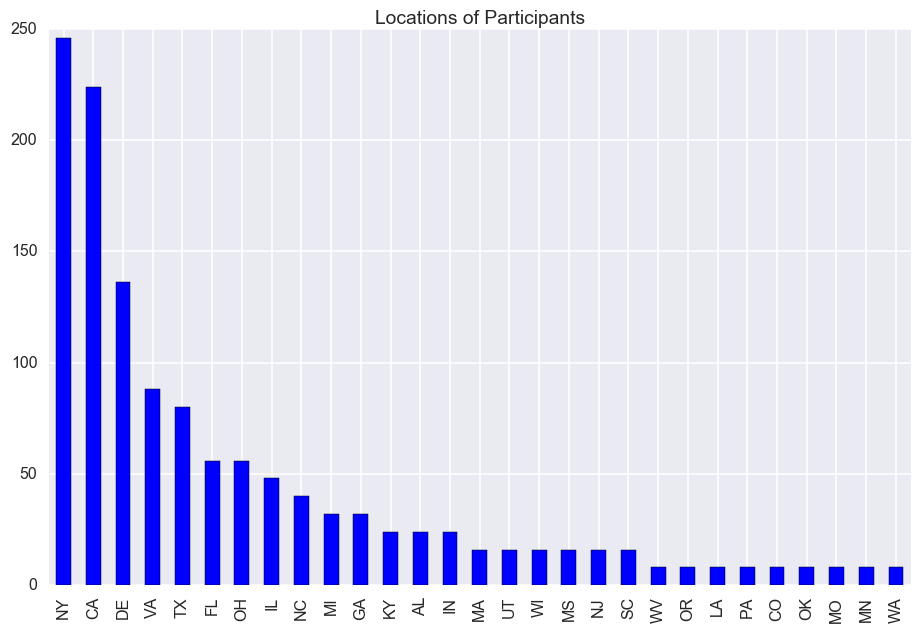
\includegraphics[width=0.32\textwidth]{location_study2} 
%   \caption{Demographics of Participants}
% \end{figure}

% \begin{figure}[h!] 
% \label{fig:locations2}
% \centering  
%   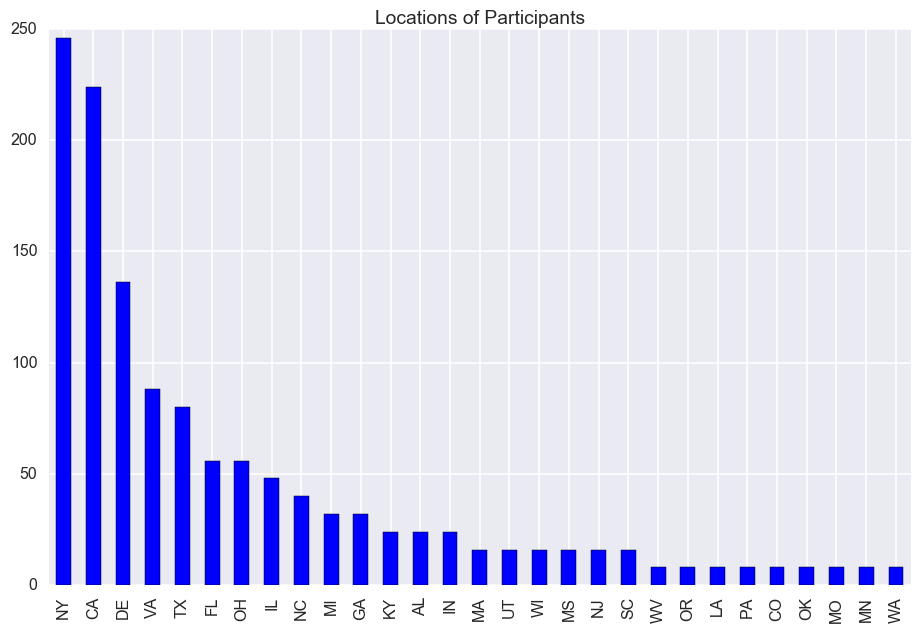
\includegraphics[width=0.9\textwidth]{location_study2} 
%   \caption{Locations of Participants}
% \end{figure}

% \begin{figure}[h!] 
% \label{fig:demographics2}
% \centering 
%   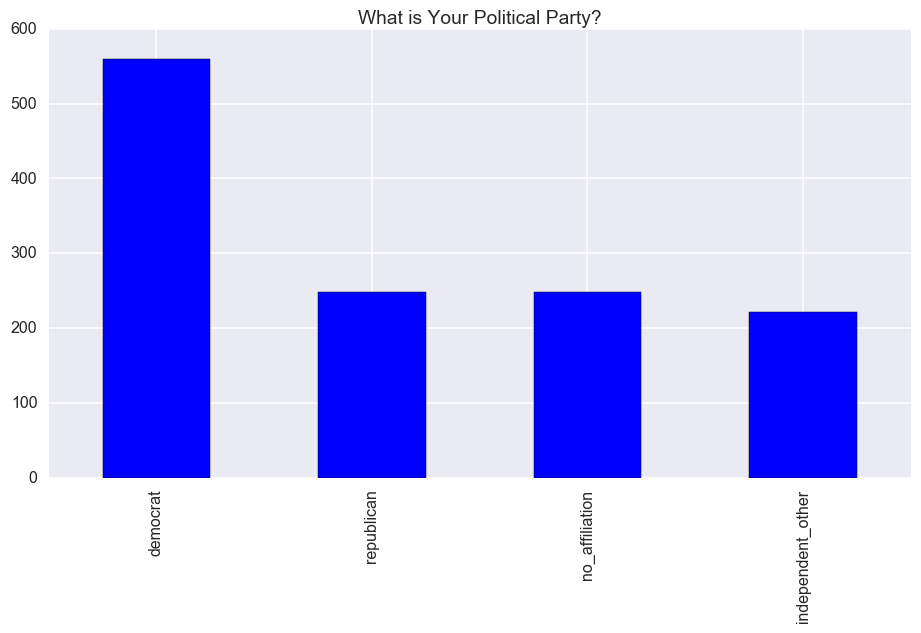
\includegraphics[width=.8\textwidth]{party_study2} 
%   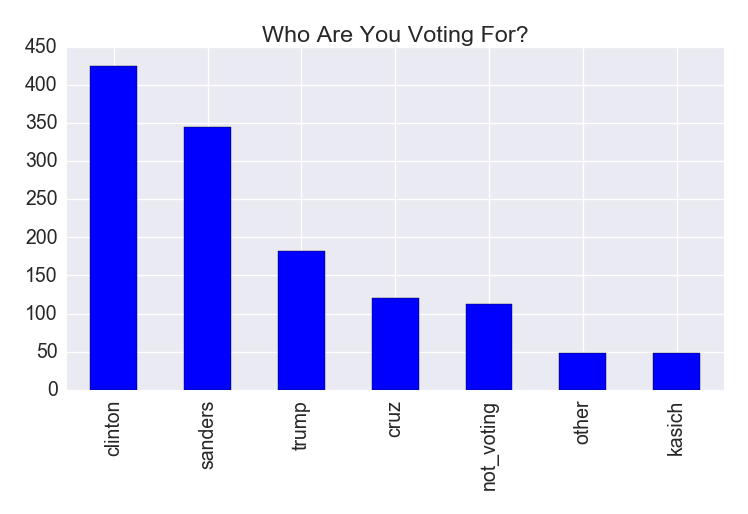
\includegraphics[width=.8\textwidth]{voting_for_study2} 
%   %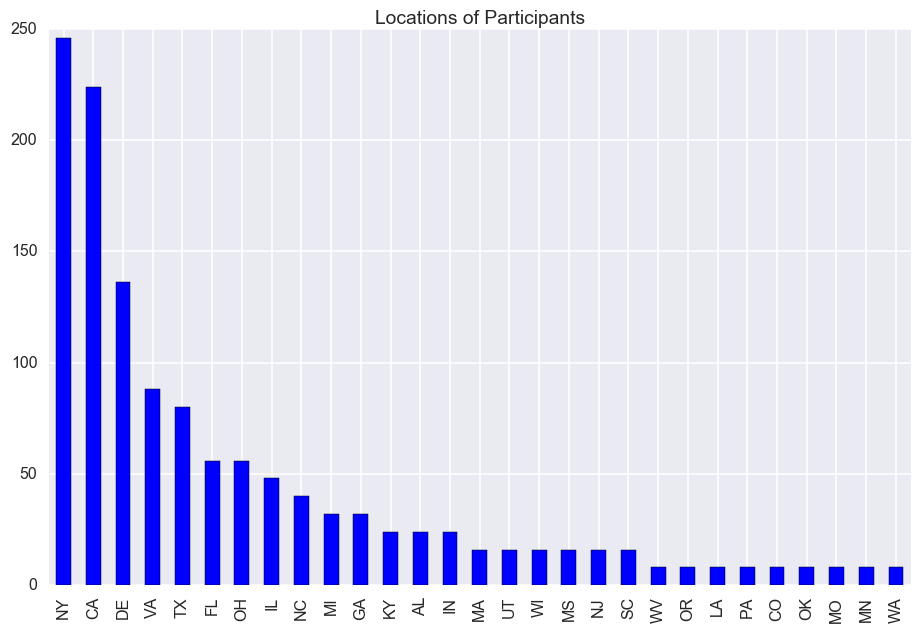
\includegraphics[width=0.32\textwidth]{location_study2} 
%   \caption{Political Affiliations of Participants}
% \end{figure}

\newpage
\subsection{Trends}
descriptive analytics of fairness and trust.



%Why did you choose trust and fairness?

 
% How did you control for quality?

  
% What kind of people signed up for your study?

% How did you recruit them? What was their incentive?

% What kind of effects were you looking for?
 
% What kind of effects did you find?

\section{Reading Level Effects}


\section{Media Brand Effects}



\section{Conclusions}

How do your trustworthiness findings line up with the findings from Pew surveys and prior work? What hypotheses did you verify from prior work?

\section{Limitations}

Our study shows significant effects that open potential new areas of experimentation while confirming past theories of how media bias is formed. In the interest of focus, our study centered around four candidates and a narrowed dataset of eight stories, but in the future could be replicated on a larger set of more diverse stories and outlets. 

Furthermore, although the contributor market on CrowdFlower is not representative of any specific region or demographic, it is also not representative of the nation at large.
